
%%\setchapterimage[6cm]{images/cabecera}
%%\setchapterpreamble[u]{\margintoc}

\chapter{Arquitectura de los Sistemas Distribuidos}
\label{ch:arq-SD}

Los sistemas que están destinados a su uso en entornos del mundo real deben diseñarse para funcionar correctamente en la mayor variedad posible de circunstancias y frente a muchas posibles dificultades y amenazas.
 
Las propiedades y los problemas de diseño de los sistemas pueden capturarse y discutirse mediante el uso de \gls{modelos  descriptivos}. Cada tipo del modelo tiene la intención de proporcionar una descripción abstracta, simplificada pero consistente de un aspecto relevante del diseño de sistemas distribuidos. Los modelos descriptivos incluyen a los \gls{modelos fisicos} y  \gls{modelos arquitectonicos}, entre otros \index{modelos descriptivos}
 
%%%%%%%%%%%%%%%%%%%%%%%%%%%%%%%%%%%%%%%%%%%%%%%%%%%%%%%%%%%%%%%%%%%%%%%%%%%%%
\section{Modelos F\'isicos}
\label{sec:fisico-SD}

Los modelos físicos son la forma más explícita de describir un sistema; ellos capturar la composición de hardware de un sistema en términos de las computadoras, dispositivos, y sus redes de interconexión.
Bajo esta óptica se puede identificar útilmente tres generaciones de distribuido sistemas \cite{Coulouris2011}. \index{modelos f\'isicos}

\begin{description}
	\item[Sistemas distribuidos tempranos] Surgieron entre 1970 y principios de 1980 en respuesta a la aparici\'on  de la tecnología de redes de área local, generalmente Ethernet. Estos sistemas constaban de entre 10 y 100 nodos interconectado por una red de área local, con conectividad a internet limitada y compatible una pequeña gama de servicios, como impresoras locales compartidas y servidores de archivos,  correo electrónico  y transferencia de archivos a través de Internet.  
	 
		\begin{tcolorbox}
		[colback=red!5!white,colframe=red!75!black,fonttitle=\bfseries,title=  Sistemas distribuidos tempranos]
			Son sistemas individuales,  en gran medida homogéneos y  la apertura no era la característica relevante. Las metas de diseño se enfocaban en la calidad del servicio \cite{Coulouris2011}
	\end{tcolorbox}
	
	
	Ejemplo de este tipo de sistema es la arquitectura \gls{cliente-servidor}  que ten\'ia  una red LAN  y un solo cliente conectado a un 	servidor. El cliente solicita  algún requerimiento al servidor, que era atendido y  luego se enviaba la respuesta a cliente. En la figura \ref{fig:ClienteServer} se ilustra  esta arquitectura
	
	\begin{figure}
		  \begin{center}%
		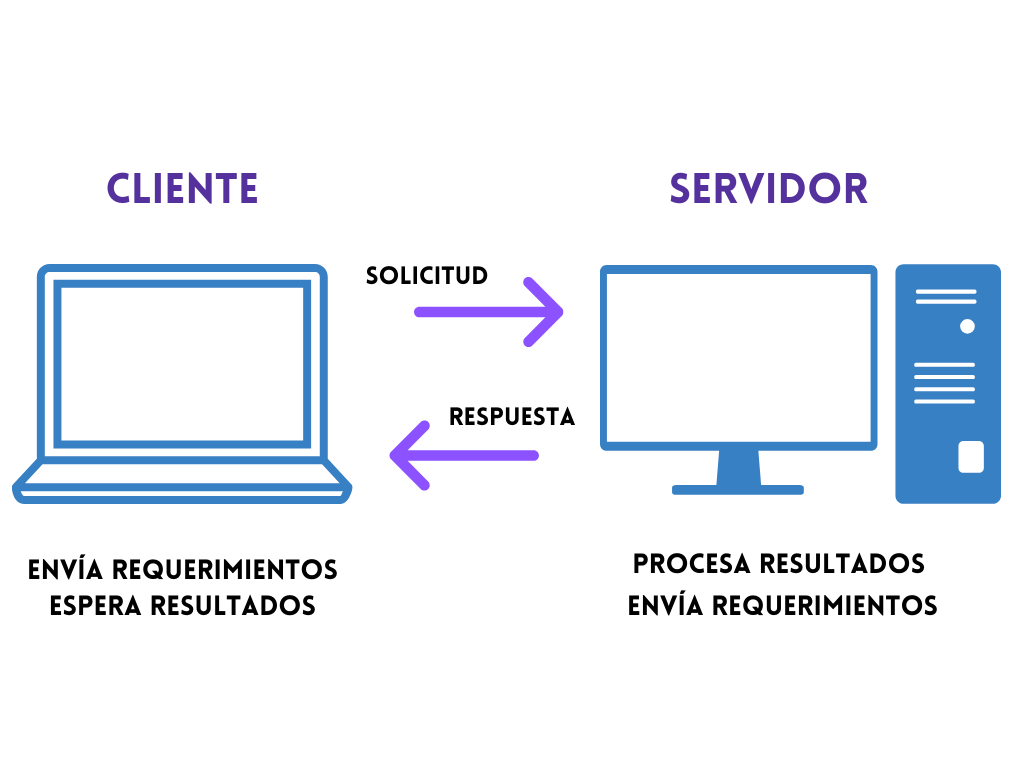
\includegraphics[width=0.8\textwidth]{2/ClienteServer.png}
		\caption{Arquitectura Cliente Servidor en red LAN}
		\label{fig:ClienteServer}
	 \end{center}
  \end{figure} 
	
	\item[Sistemas distribuidos a escala de internet.]  Comenzaron a surgir en  1990 en respuesta al crecimiento de Internet. En estos sistemas la infraestructura física subyacente consiste en un modelo físico como un conjunto extensible de nodos interconectados por una red de redes (Internet).  Incorporan grandes cantidades de nodos y proporcionar servicios de sistema distribuido para organizaciones globales y en toda la organización.   
	
 
	
		\begin{tcolorbox}
		[colback=red!5!white,colframe=red!75!black,fonttitle=\bfseries,title=Sistemas distribuidos a escala de internet]
		Son sistemas heterogéneos en términos de redes, arquitectura de computadoras, sistemas operativos, idiomas empleados y equipos de desarrollo involucrados. \\Los nodos pueden ser \gls{nodos estaticos},  \gls{nodos discretos} y \gls {nodos autonomos}.
	\end{tcolorbox}
	
	
	
	Ejemplos de modelos físicos de esta época están en: 
	\begin{itemize}
		\item Arquitectura cliente-servidor. Puede presentar varios clientes conectados a un servidor, como el de la figura \ref{fig:ClienteServerco}, varios clientes y 	servidores conectados a internet y conversando entre ellos. \index{cliente-servidor}
		
		\begin{figure} 
			\begin{center}%
			 
			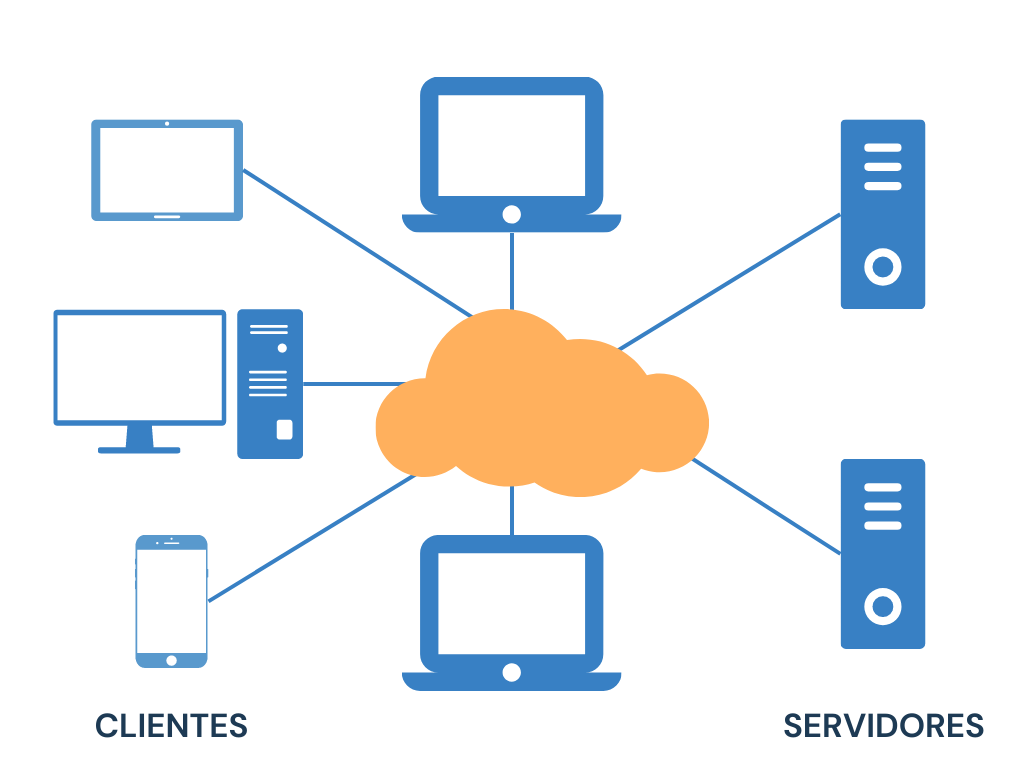
\includegraphics[width=0.8\textwidth] {2/ClienteServerComp.png}
			\caption{Arquitectura Cliente Servidor}
			\label{fig:ClienteServerco}
				\end{center}
	  \end{figure} 
		
		\item Arquitectura P2P. Constituido por un grupo de m\'aquinas o nodos conectados entre s\'i, ver figura \ref{fig:p2p}. Cada nodo cumple las mismas fuciones y tiene las mismas responsabilidades que el resto de los nodos. \index{P2P}
			
		\begin{figure}[h]%
				\begin{center}
			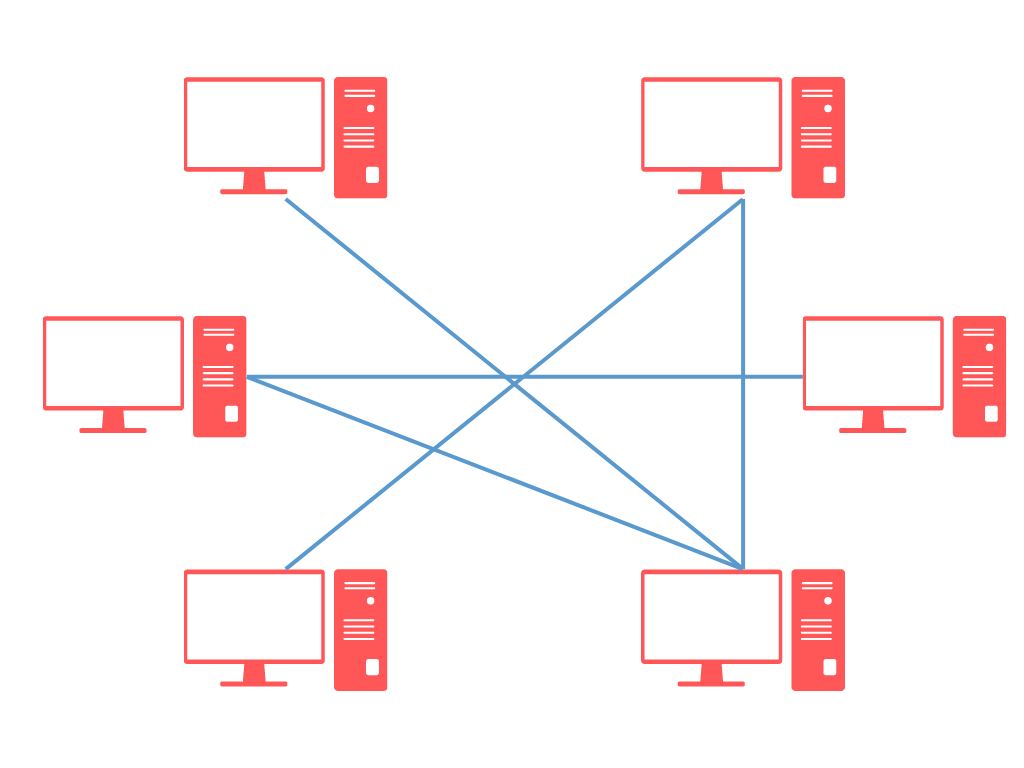
\includegraphics[width=0.8\linewidth]{2/P2P.png}
			\caption{Arquitectura Punto a Punto}
			\label{fig:p2p}
				\end{center}
		\end{figure}  
		
 		Algunas aplicaciones con esta arquitectura:  \href{https://ares.com/}{Ares}, 
				\href{https://bitcoin.org/es/}{bitcoin},  \href{https://edonkey-2000/}{eDonkey}.

	\end{itemize}
	\item[Sistemas distribuidos contemporáneos] Las tendencias claves, interoperabilidad y \gls{sistemas abiertos},  han dado como resultado importantes desarrollos como:
	
	\begin{itemize}
		\item Informática móvil.  Donde los nodos, tales como las computadoras portátiles o los teléfonos inteligentes, pueden moverse de una ubicación a otra en un sistema, lo que lleva a la necesidad de capacidades adicionales como el \gls{descubrimiento de servicios} y apoyo a la interoperación espontánea. \index{inform\'atica m\'ovil} \index{descubrimiento de servicios}
		
		\item Computación ubicua. La \gls{computacion ubicua} ha llevado a pasar de nodos discretos a arquitecturas donde las computadoras están incrustadas en objetos cotidianos. \index{computaci\'on ubicua}
		
		\item Computación en la Nube. En \gls{computacion en la nube}. y, en particular, las arquitecturas de clúster ha llevado a un movimiento que va  desde nodos autónomos que realizan un rol determinado a grupos de nodos que juntos brindan un servicio específico. \index{computaci\'on en la nube}
		
		Algunas empresas que prestan este servicio: \href{https://cloud.google.com/}{Google}  y 				\href{https://aws.amazon.com/es/}{Amazon}.
	
	\end{itemize}

	\item[Sistemas de Sistemas Distribuidos.] Son  sistemas distribuidos complejos y a gran escala (arquitecturas físicas y redes de redes). Un sistema de sistemas se puede definir como un sistema complejo que consiste en una serie de subsistemas que son sistemas por derecho propio y que se unen para realizar una tarea o tareas particulares. 

	Ejemplos son sistemas que usan bases de datos distribuidas en tiempo real, como en \cite{Sakaki2010} donde se relaciona  las publicaciones que hacen  las personas en Twitter (tweets) relacionadas con un terremoto, lo que permite detectar rápidamente la ocurrencia de un terremoto y proponen un algoritmo para monitorear tweets y detectar un evento objetivo.  
	
	Y en \cite{Basha2008} presentan un sistema basado en  redes de sensores ambientales predictivos donde se presenta una aplicación para predecir de inundaciones de ríos.	
\end{description}
%%%%%%%%%%%%%%%%%%%%%%%%%%%%%%%%%%%%%%%%%%%%%%%%%%%%%%%%%%%%%%%%%%%%

\section{Modelos Arquitect\'onicos }
\label{sec:mod-arquitec}
\index{modelos arquitect\'onicos}

Los modelo arquitectónicos clasifican su contenido en componentes de la arqiuitectura: entidades, paradígmas de comunicación, roles y responsabilidades, y correspondencia con la infraestructura física \cite{Coulouris2011}.

A  continuación se describe los modelos arquitect\'onicos de los sistemas distribuidos de acuerdo a esa caracterización.

\subsection {Entidades}
\label{subsec:entidades}
\index{entidades}
Las entidades presentes en un sistema distribuidos son: procesos, nodos, hilos, componentes, servicios web. Seguidamente, se describen.

\begin{description}	
	\item [Procesos] Conducen a visión  predominante de un sistema distribuido como \gls{procesos} acoplados y paradigmas de comunicación entre procesos.  \index{procesos}
	Por ejemplo\cite{Tanenbaum2007},  en la figura \ref{fig:Arq-procesos} se ilustra la organización de una base de datos una red de monitoreo y los procesos que se ejecutan en ella, en el lugar del operador (a), o en los sensores (b). 
	
	\begin{figure}%
			\begin{center}
		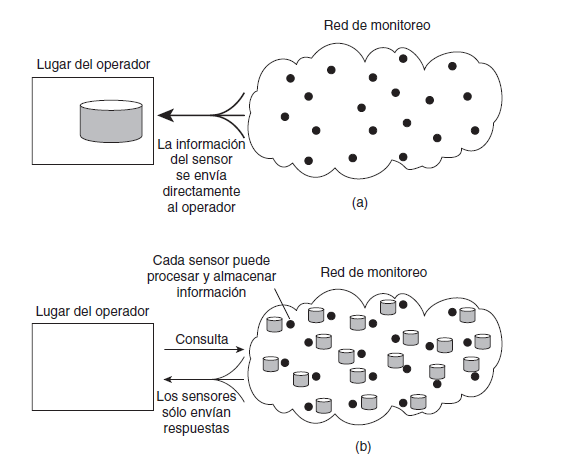
\includegraphics[width=0.8\linewidth]{2/procesos.png}
		\caption{Organización de una base de datos para una red de monitoreo, 	mientras se almacena y procesa información (a) sólo en el lugar del operador, 	o (b) sólo en los sensores. Tomado de \cite{Tanenbaum2007}}
		\label{fig:Arq-procesos}
			\end{center}
	  \end{figure} 
	
	\item [Nodos]  En algunos entornos primitivos, como las redes de sensores,  los sistemas operativos pueden que no admitan abstracciones de proceso  y, por lo tanto, las entidades que se comunican en este tipo de sistemas son \gls{nodos}. \index{nodos}
	La Figura \ref{fig:Arq-nodos} muestra la organización de los nodos en la arquitectura de Chord \cite{Stoica2001}, un protocolo y algoritmo para sistemas P2P con \gls{tablas hash distribuidas}   y que proporcina un servicio de búsqueda descentralizado que almacena pares clave/valor para esas redes. 
	
 		
 		\begin{tcolorbox}
 			[colback=red!5!white,colframe=red!75!black,fonttitle=\bfseries,title=Chord]
 				Es un protocolo y algoritmo para la implementaci\'on de tablas hash distribuidas para sistemas P2P. Ver \href{https://github.com/sit/dht/wiki}{Chord} 
 		 
 		\end{tcolorbox}
 		
	
	\begin{figure}%
			\begin{center}
		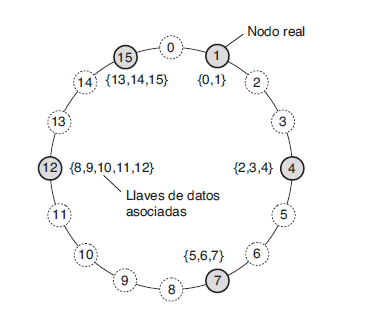
\includegraphics[width=0.8\linewidth]{2/nodos}
		\caption{Mapeo de elementos de datos hacia nodos organizados en Chord. Tomado de \cite{Tanenbaum2007} }
		\label{fig:Arq-nodos}
			\end{center}
	  \end{figure} 
		
	\item [Hilos] En la mayoría de los entornos de sistemas distribuidos, los procesos se complementan con \gls{hilos}, que  son los puntos finales de la comunicación. \index{hilos}
	En la Figura {\ref{fig:Arq-hilos}} se presenta   los hilos  que se establecen en la  comunicaci\'on del cliente y el servidor con el \gls{protocolo solicitud-respuesta}.
	
	\begin{figure}%
			\begin{center}
		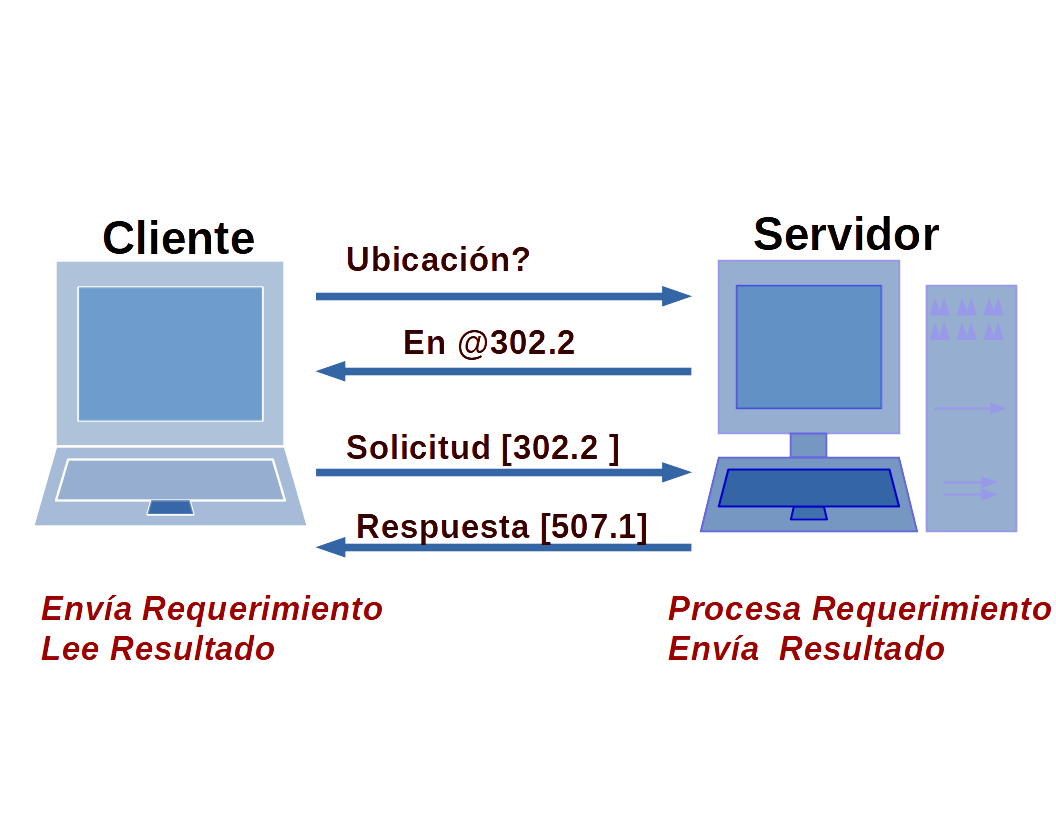
\includegraphics[width=0.8\linewidth]{2/hilos.png}
		\caption{Hilos en Arquitectura Cliente Servidor}
		\label{fig:Arq-hilos}
			\end{center}
	   \end{figure} 
	
	\item[Objetos]   En el enfoque de sistemas distribuido basado en \gls{objetos}, un cálculo consiste en una serie de objetos interactivos que representan unidades  para el dominio del problema dado. Se accede a los objetos a través de interfaces, con un lenguaje de definición de interfaz asociado ( \textit{interface definition language, IDL}) que proporciona un especificación de los métodos definidos en un objeto. 
	\index{objeto} \index{Corba}
	Por ejemplo, en la Figura \ref{fig:Arq-object}, se muestra la constituci\'on de la arquitectura de \gls{Corba}, detallando los objetos y sus funciones \cite{Corba2022}. 

	\begin{figure}  
		\begin{center}%
		\includegraphics[width=0.8\linewidth]{2/Arq-object.png}
		\caption{Componentes de la arquitectura CORBA.}
		\label{fig:Arq-object}
	 \end{center}
  \end{figure} 
	
	\item [Componentes.]  \index{componentes}
%%	Se parecen a los objetos porque ofrecen abstracciones orientadas a problemas para construir sistemas distribuidos y también son accedido a través de interfaces. La diferencia es que los \gls{componentes} especifican no solo sus interfaces, también las supuestos que hacen en términos de otros componentes/interfaces que deben estar presentes para que un componente cumpla su función. \index{componentes} 
	
	En los \gls{componentes} de software, cada componente es  una unidad de composición con interfaces especificadas contractualmente y dependencias de contexto explícitas únicamente. Esto indica que no hay dependencias implícitas. 
	
	Los componentes de software son como objetos distribuidos en el sentido de que están encapsulados en 	unidades de composición, pero un componente dado especifica tanto sus interfaces proporcionadas al mundo exterior y sus dependencias de otros componentes en el entorno distribuido  \cite{Szyperski2002}.	
	La Figura \ref{fig:Arq-componente} muestra la arquitectura de un sistema de archivos simple que proporciona una interfaz a otros usuarios y, a su vez, 	que requiere conexión a un componente de servicio de directorio y un componente de servicio de archivo plano.
	
	\begin{figure} 
		\begin{center}%
		\includegraphics[width=0.8\linewidth]{2/Arq-componente.png}
		\caption{Arquitectura de software basado en componentes. Tomado de \cite{Coulouris2011}}
		\label{fig:Arq-componente}
	 \end{center} 
 \end{figure} 
	
	\item [Servicios Web.]  \index{servicios web}  
	Los \gls{servicios web} están estrechamente relacionado con objetos y componentes,  adoptando un enfoque basado en la encapsulación de comportamiento y acceso a través de interfaces. Están integrados en la \textit{World Wide Web}, utilizando estándares web para representar y descubrir servicios \cite{Erl2007}. 
	
	En \cite{W3C2022} lo definen como un sistema software diseñado para soportar la interacción máquina-a-máquina, a través de una red, de forma interoperable. Cuenta con una interfaz descrita en un formato procesable por un equipo informático (específicamente en WSDL), a través de la que es posible interactuar con el mismo mediante el intercambio de mensajes SOAP, típicamente transmitidos usando serialización XML sobre HTTP conjuntamente con otros estándares web.
	 
	
		\begin{tcolorbox}
		[colback=red!5!white,colframe=red!75!black,fonttitle=\bfseries,title=Servicios WEB]
			Servicios WEB, SOA, es un est\'andard de la OMG. Puede verlo en \href{https://www.omg.org/technology/readingroom/SOA.htm} {SOA}	
		\end{tcolorbox}
	

%	El esquema de la Figura \ref{fig:Arq-servicio} detalla el servicio Agente de Viaje y su integraci\'on con otros servicios. Esta combinacio\'on de servicios proporciona beneficios a los usuarios de los mismos: considere el hecho de que muchas personas reservan vuelos, hoteles y autos de alquiler para viajes en línea utilizando una variedad de sitios web diferentes. Si cada uno de estos sitios web proporcionara una interfaz de servicio web estándar, entonces un "servicio de agente de viajes" podría utilizar sus operaciones para proporcionar al viajero una combinación de estos servicios.
	
%%	\begin{figure}   	\begin{center}%
%%		\includegraphics[width=0.8\textwidth]{Arq-servicio.png}
%%		\caption{El servicio Agente de Viaje combinado con otros servicios Web. Tomado de %%\cite{Couloris2011}} 		\label{fig:Arq-servicio} 	 \end{center} \end{figure} 
	
\end{description}

\subsection{Paradigma de comunicación }
\label{subsec:paradigmas} \index{paradigmas de comunicaci\'on}

Considere tres tipos de paradigma de comunicación: comunicación entre procesos, Invocación remota y comunicación indirecta \cite{Steen2017} \cite{Elshebani2009} \cite{Silcock1995}  .

\begin{description}
	\item[Comunicación entre procesos] Se refiere al soporte de bajo nivel  para comunicación entre procesos en sistemas distribuidos . \index{procesos} 
	\index{pase de mensaje} \index{socket} \index{multidifusi\'on}
	
%%	 
		  
	
		\begin{tcolorbox}
		[colback=green!5!white,colframe=green!75!black,fonttitle=\bfseries,title=Comunicación entre procesos ]
			\begin{itemize}
			\item Pase de mensaje
			\item Sockect
			\item Multidifusi\'on
			\end{itemize} 	
	\end{tcolorbox}
	
	
		
	\item[Invocación remota] Representa el paradigma de comunicación más común en sistemas distribuidos, cubren una gama de técnicas basadas en un intercambio bidireccional entre entidades comunicantes. \index{invocaci\'on remota}
	
		    	 
	
		\begin{tcolorbox}
		[colback=red!5!white,colframe=red!75!black,fonttitle=\bfseries,title=Invocación remota]
		Incluye:
		\begin{itemize}
			\item Protocolo Solicitud-respuesta  	
			\item Llamada a procedimientos remotos  	
			\item Llamada a m\'etodos remotos
		\end{itemize} 		
	\end{tcolorbox}
	
	
	

	\begin{description}
		
		\item[Protocolo solicitud-respuesta].   El \gls{protocolo solicitud-respuesta} es un patrón impuesto en un servicio subyacente de transmisión de mensajes para admitir la informática cliente-servidor.  Este paradigma es bastante primitivo y  se usa  en sistemas embebidos donde el rendimiento es primordial. El  enfoque también se utiliza con el protocolo HTTP. \index{protocolo solicitud-respuesta}
		
		\item[Llamadas a procedimiento remoto].  \textit{(Remote Procediment Call, RPC)} es computación cliente-servidor con servidores que ofrece un conjunto de operaciones a través de un interfaz de servicio y clientes que llaman a estas operaciones directamente como si estuvieran disponibles en la zona.  
		\index{llamadas a procedimientos remotos}
				\index{RPC}
		
		\item [Invocación de métodos remotos]. La invocación de métodos remotos \textit{(Remote Method Invocation, RMI)} se parece mucho a llamadas a procedimiento remoto pero en un mundo de objetos distribuidos  
		 \index{paradigmas de comunicaci\'on!invocaci\'on a m\'etodos remotos}
		 		\index{RMI}
	
	\end{description}
	
	\item[Comunicaci\'n Indirecta] Se realiza a  través de una tercera entidad, lo que permite un fuerte grado de desacoplamiento entre remitentes y receptores. En este paradigma los remitentes de los mensajes no necesitan saber a quién están enviando mensajes; y no es necesario que los emisores y los receptores existan al mismo tiempo. 
	\index{desacoplamiento en espacio} \index{desacoplamiento en tiempo}
	
%%	 
		  
		
		
			\begin{tcolorbox}
			[colback=green!5!white,colframe=green!75!black,fonttitle=\bfseries,title=Comunicaci\'on indirecta ]
				Comprende los siguientes 
			\begin{itemize}
				\item Comunicación grupal.  				
				\item Sistema Publicación-Suscripción.
				\item Cola de Mensaje.
				\item Espacios de Tupla.
				\item Memoria compartida Distribuida.
			\end{itemize}
			\end{tcolorbox}
		
	
	
	\begin{description}		
		\item[ Comunicaci\'on grupal.]  La \gls{comunicacion grupal} se basa en la abstracción de un grupo que está representado en el sistema por un identificador de grupo.  \index{comunicaci\'on grupal}
		
		\item[Sistemas de publicaci\'on-suscripci\'on.]  Los sistemas pub-sub (\gls{pub-sub})  donde los productores   distribuyen elementos de informacion de interes o eventos, a los comsumidores (llamado tambi\'en, sistemas basados en eventos distribuidos). Ver esquema de la arquitectura en la Figura \ref{fig:Arq-pubsub}.   \index{ publicaci\'on-suscripci\'on}  \index{pub-sub}
		
		\begin{figure}[h]
			  \begin{center}%
			\includegraphics[width=0.8\linewidth]{2/arq-pub-sub.png}
			\caption{Arquitectura Publicaci\'on Suscripci\'on. }
			\label{fig:Arq-pubsub}
		 \end{center} 
	 \end{figure} 
		
		
		\item[Colas de mensajes.]  Servicio punto a punto mediante el cual el productor pueden enviar mensajes a una cola específica y el consumidor puede recibir mensajes de la cola o ser notificado de la llegada de nuevos mensajes en el cola.
		Ver Figura \ref{fig:Arq-cola}.
		\index{cola de mensaje}
		
		\begin{figure}[h] 
			\begin{center}%
			\includegraphics[width=0.8\linewidth]{2/arq-cola.png}
			\caption{Arquitectura Colas de Mensajes.}
			\label{fig:Arq-cola}
		 \end{center} 
	 \end{figure} 
		
		\item[Espacios de tupla.] Los procesos pueden colocar elementos arbitrarios de datos estructurados o tuplas, en un espacio de tuplas persistente;  otros procesos pueden leer o eliminar tales tuplas del espacio de tuplas especificando patrones de interés.    \index{espacio de tuplas}
		
		\item[Memoria compartida distribuida.]  Proporciona un abstracción para compartir datos entre procesos que no comparten memoria física. A los programadores se les presenta una abstracción  de lectura o escritura de estructuras de datos (compartidas) como si estuvieran en sus propios espacios de direcciones locales.   \index{memoria compartida distribuida}
		
	\end{description} 	 	
	
\end{description}


\subsection { Roles y responsabilidades} 
\label{subsec:roles}
Los estilos de arquitectura seg\'un los roles y responsabilidades que cumplen los nodos,  incluyen: 
\begin{itemize}
	\item Rol que juegan los nodos ya sea como clientes y servidores en la arquitectura cliente-servidor. 
	\item Mismas funciones que cumplen los nodos en una arquitectura p2p, por ejemplo (sección \ref{sec:fisico-SD}).
	\item Rol como publicadores o suscriptores de eventos en una arquitectura pub-sub (ver descripci\'on en sección \ref{sec:fisico-SD}).
	\item Rol como productores o consumidores de mensajes en una arquitectura basada en colas (ver descripci\'on en sección \ref{sec:fisico-SD} ).
	
\end{itemize}

\subsection{Correspondencia con la infraestructura física distribuida}
\label{subsec:corresp}

En esta clasificaci\'on se considera  cómo las entidades, objetos o servicios se asignan o forman parte de la infraestructura física distribuida subyacente. Se exploran tres aspectos \cite{Coulouris2011}, \cite{Limoncelli2014}:

\begin{itemize}
	\item Elementos que conforman la arquitectura
	\item Patrones que usa la arquitecura  y
	\item Soluciones basadas en middleware 
\end{itemize}


\paragraph{Elementos de la Arquitectura}

	 	\begin{tcolorbox}
		[colback=red!5!white,colframe=red!75!black,fonttitle=\bfseries,title= Elementos de la Arquitectura]
			Comprende los siguientes 
		\begin{itemize}
			\item Correspondencia de servicios con servidores.  				
			\item Memoria Cache.
			\item Código Móvil.
			\item Agentes Móviles.
		\end{itemize}
	\end{tcolorbox}
	
	
	
	 
\begin{description}
	\item[ Correspondencia de servicios con servidores.] Los servicios pueden implementarse como varios servidores de procesos en computadoras separadas que interactúan según sea necesario para proporcionar un servicio a procesos del cliente. En la Figura \ref{fig:arq-multiserver} se muestra un ejemplo. \index{servidores m\'utiples}
	
	
	\begin{figure}[h]  
		\begin{center}%
		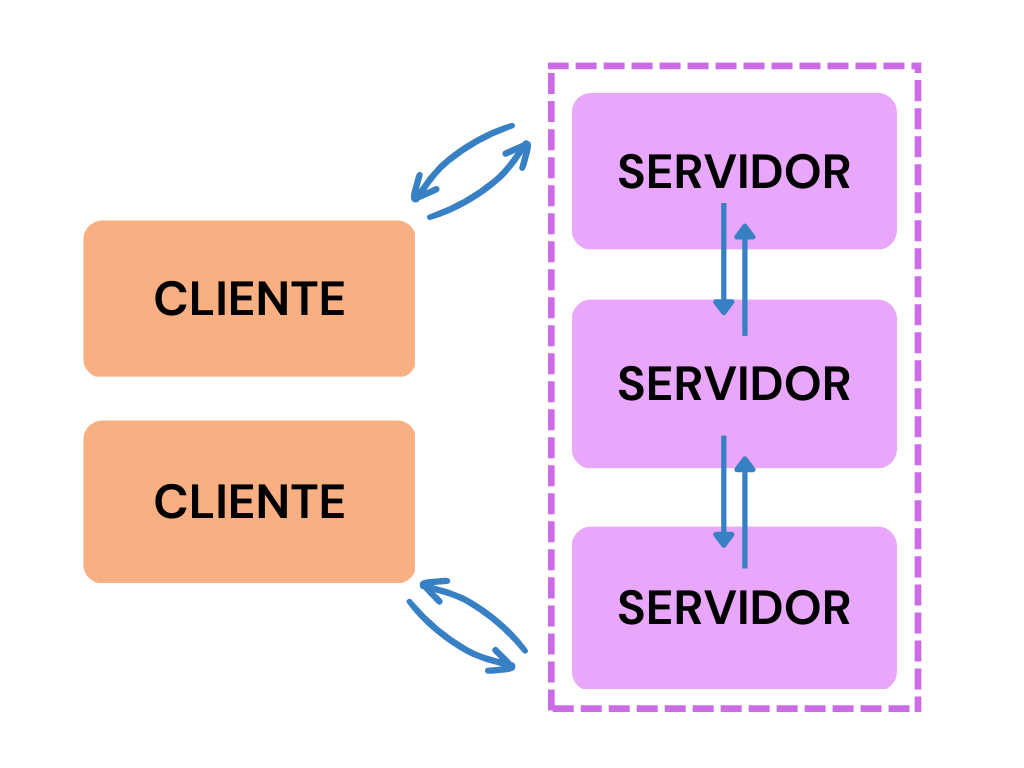
\includegraphics[width=0.8\linewidth]{2/Arq-mult-server.png}
		\caption{Arquitectura con m\'ultiples servidores. Tomado de \cite{Coulouris2011} }
		\label{fig:arq-multiserver}
	 \end{center} 
 \end{figure} 
	
	
	\item[Cache.] Los navegadores web mantienen un \gls{cache} 
	con las páginas web visitadas recientemente y otros recursos web en el sistema de archivos local del cliente, utilizando
	una solicitud HTTP para verificar con el servidor original que las páginas en caché están actualizadas. Un \gls{servidor proxy} web (ver Figura \ref{fig:arq-webproxy}) proporciona un caché compartido de recursos web para las máquinas cliente en un sitio o en varios sitios. \index{cach\'e}
	
	\begin{figure}[h]
		\begin{center}%
		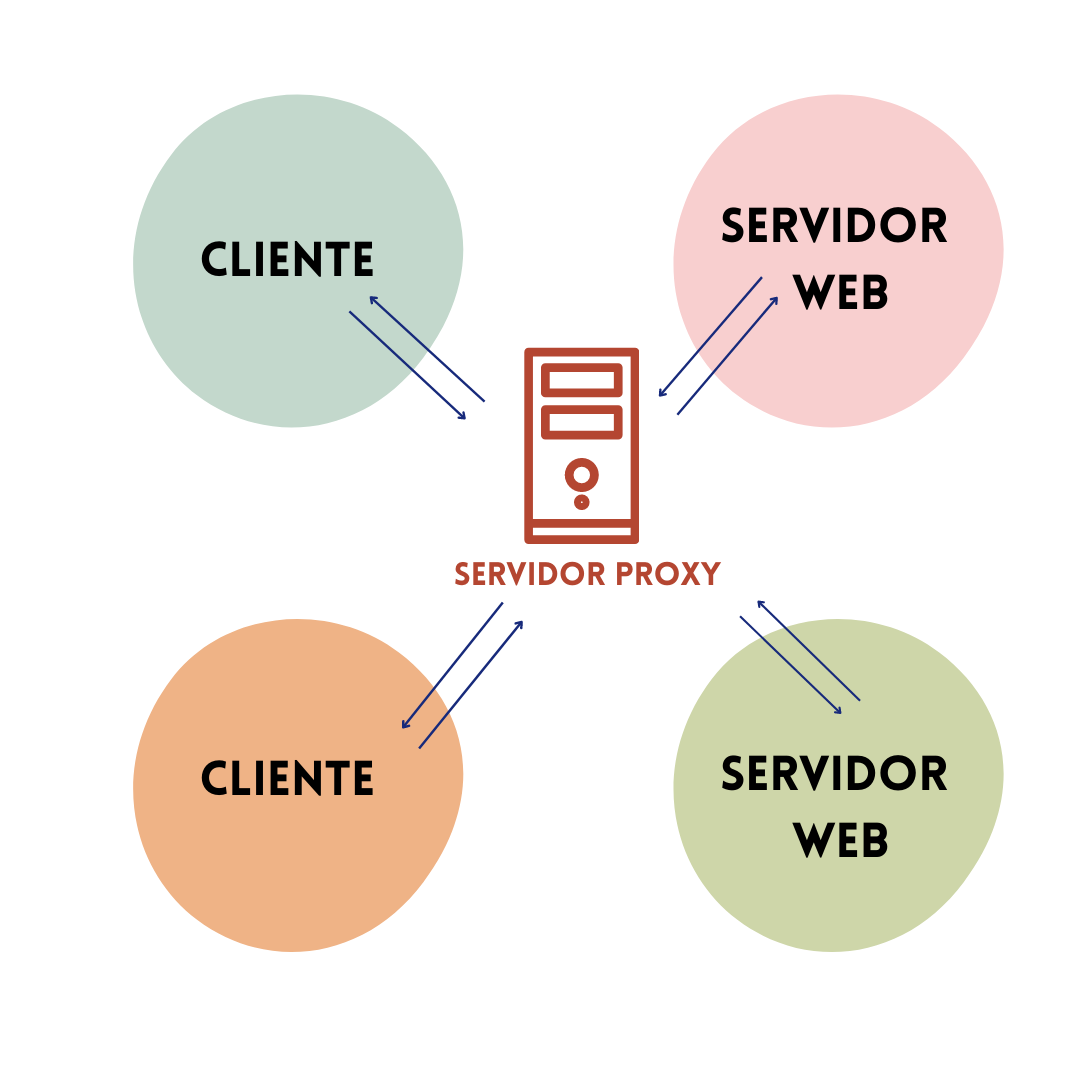
\includegraphics[width=0.8\linewidth]{2/Arq-web-proxy.png}
		\caption{Arquitectura web proxy. }
		\label{fig:arq-webproxy}
	 \end{center} 
 \end{figure} 
	
	\item[ C\'odigo m\'ovil] El \gls{applet}  es un ejemplo   de código móvil: el usuario que ejecuta un navegador selecciona un enlace a un subprograma cuyo código se almacena en un servidor web; el código se descarga en el navegador y lo ejecuta , como se muestra en la Figura \ref{fig:arq-webapplet}. \index{c\'odigo m\'ovil} \index{applet}
	
	\begin{figure}  
		\begin{center}%
		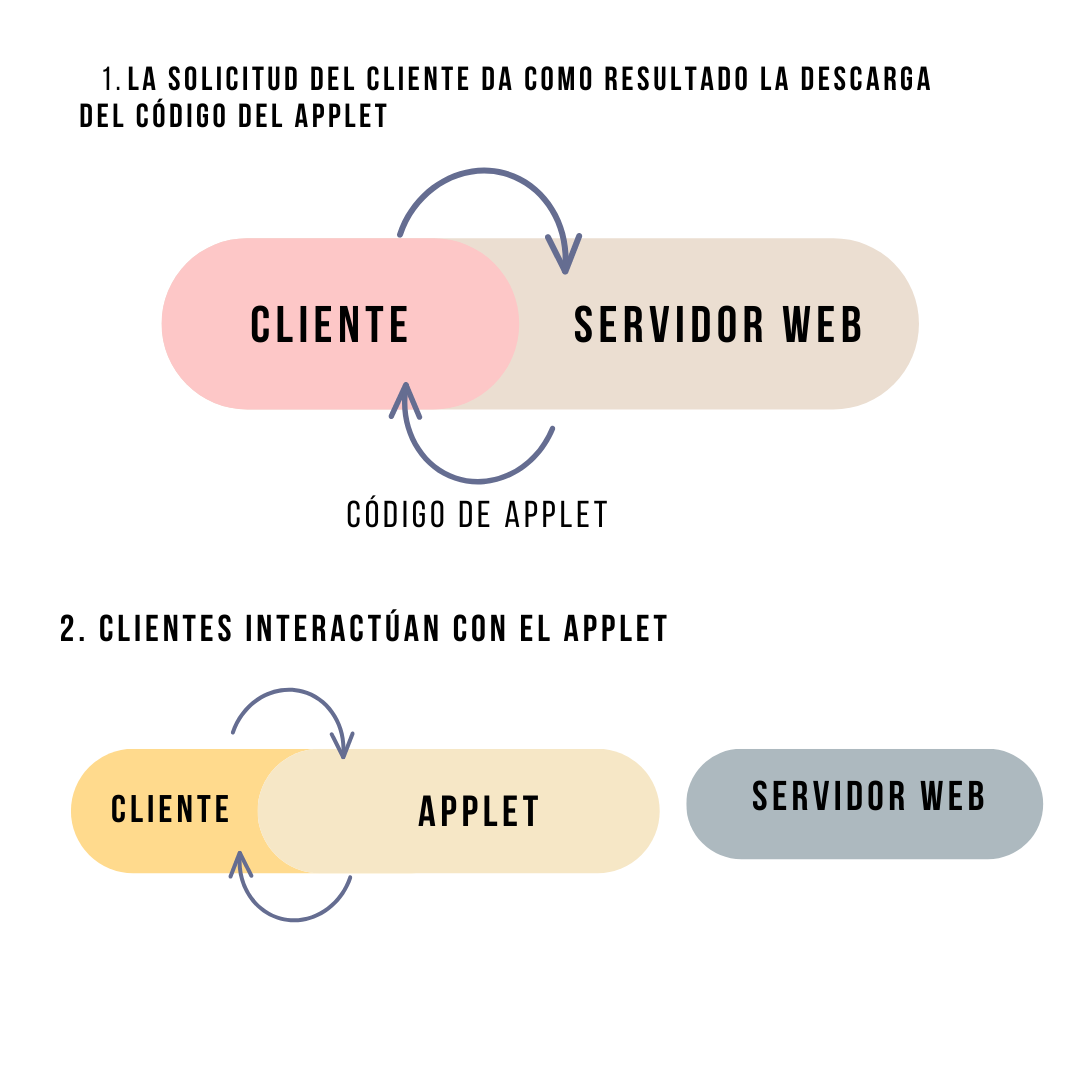
\includegraphics[width=0.8\linewidth]{2/Arq-web-applet.png}
		\caption{Arquitectura web applet.  }
		\label{fig:arq-webapplet}
	 \end{center} 
 \end{figure} 
	
	\item[Agentes m\'oviles] El \gls{agente movil} puede realizar   invocaciones a los recursos locales en cada sitio que visita, por ejemplo, acceder a entradas individuales de la base de datos.  
	Los agentes móviles pueden usarse para instalar y mantener software en las computadoras dentro de una organización o para comparar los precios de productos de varios proveedores 	visitando el sitio de cada proveedor y realizando una serie de operaciones de base de datos.  
\end{description} \index{agente m\'ovil}
%%%%%%%%%%%%%%%%%%%%%%%%%%%%%%%%%%%%%%%%

\paragraph{Patrones de Arquitectura}

Los patrones arquitectónicos \cite{Pressman2019}  dan una descripción de los elementos y el tipo de relación que tienen junto con un conjunto de restricciones. Un patrón arquitectónico expresa un esquema de organización estructural esencial para un sistema de software, que consta de subsistemas, sus responsabilidades e interrelaciones.
No son necesariamente soluciones completas en sí mismas, sino que
ofrecen conocimientos parciales que, cuando se combinan con otros patrones, llevan al diseñador a una  solución para un dominio de problema dado.

 
	\begin{tcolorbox}
	[colback=red!5!white,colframe=red!75!black,fonttitle=\bfseries,title=  Patrones de Arquitectura]
	Se presentan los siguientes:
	\begin{itemize}
		\item Capas
		\item Arquitectura de capas
		\item Cliente flacos
		\item Patrón Proxy
		\item Bokerage 	
		\item Balanceador de carga con réplicas (\textit{backend})   
		\item Servidor con réplicas  
		\item \'Arbol de servidores		
	\end{itemize} 
	\end{tcolorbox}




\begin{description}
	\item[Capas] En un enfoque por capas, un sistema complejo se divide en varias capas, con un capa dada haciendo uso de los servicios ofrecidos por la capa siguiente. La capa referida ofrece una abstracción de software, con capas superiores que desconocen detalles de su implementación, o  de cualquier otra capa debajo de ellos.
	En términos de sistemas distribuidos, esto equivale a una organización vertical de servicios en capas de servicio.  Ejemplo de esta estructura es el \gls{middleware}. \index{capas}
	
	\item[Arquitectura de capas] Las arquitecturas de capas 
	es una técnica para organizar la funcionalidad de una capa determinada y colocarla en servidores apropiados y, como consideración secundaria, en los nodos físicos. Esta  técnica se asocia más comúnmente con la organización de aplicaciones y servicios. Por ejemplo, en la \ref{fig:Arq-capas} se observa una arquitectura de dos capas, cliente y servidor; mientras la Figura \ref{fig:Arq-capas-3} es el esquema de una arquitectura de tres capas: cliente, servidor y servidor de base de datos.
	\index{arquitectura de capas}
	
	\begin{figure}  
		\begin{center}%
		\includegraphics[width=0.8\linewidth]{2/arq-capas.png} 
		\caption{Arquitectura de capas de dos niveles.}
		\label{fig:Arq-capas}
	 \end{center} 
 \end{figure} 
	
	\begin{figure}  
		\begin{center}%
 	\includegraphics[width=0.8\linewidth]{2/arq-capas-2.png}
	\caption{Arquitectura de capas de tres niveles.}
	\label{fig:Arq-capas-3}
 \end{center} 
\end{figure} 

	
	\item[Clientes flacos] La tendencia en la computación distribuida es alejar la complejidad del dispositivo del usuario final hacia los servicios en Internet. Esto es más evidente en  la computación en la nube,  pero también se puede ver en la arquitectura de niveles.  Esta tendencia ha suscitado el interés en  \gls{cliente ligero}, que  permite el acceso a sofisticados servicios en red, proporcionados por una solución en la nube, con pocas suposiciones o demandas en el dispositivo del cliente, entre otros.  La Figura \ref{fig:Arq-flaco}  ilustra un cliente ligero que accede a un servidor informático a través de Internet.
	\index{clientes flacos}
	
	\begin{figure}[h]
		  \begin{center} %
		\includegraphics[width=0.8\linewidth]{2/arq-clienteFlaco.png}
		\caption{Arquitectura de cliente ligero. }
		\label{fig:Arq-flaco}
	 \end{center} 
 \end{figure} 
	
 
	
%	\begin{description}
		\item[\textit{Patron Proxy}] El \gls{patron proxy} es un patrón  recurrente en sistemas distribuidos, diseñados  para apoyar la transparencia de la ubicación en llamadas de procedimiento remoto (RPC) o invocación del método (RMI).  Es un intermediario entre un objeto y el resto que lo invoque.  
		
		\item[\textit{Brokerage}]
		  
	 	 El uso de corredores o \textit{brokerage}  en servicios web puede verse  como un patrón que admite la interoperabilidad en infraestructuras distribuidas potencialmente complejas.	
		 Este patrón consta del trío de proveedores de servicios, solicitante de servicios y corredor de servicios (un servicio que coincide con los servicios prestados a los solicitados), como se muestra en la Figura \ref{fig:brokerage}.
		 
		 
		
		%%	
	
				
		\begin{figure}[h]  
			\begin{center}%
			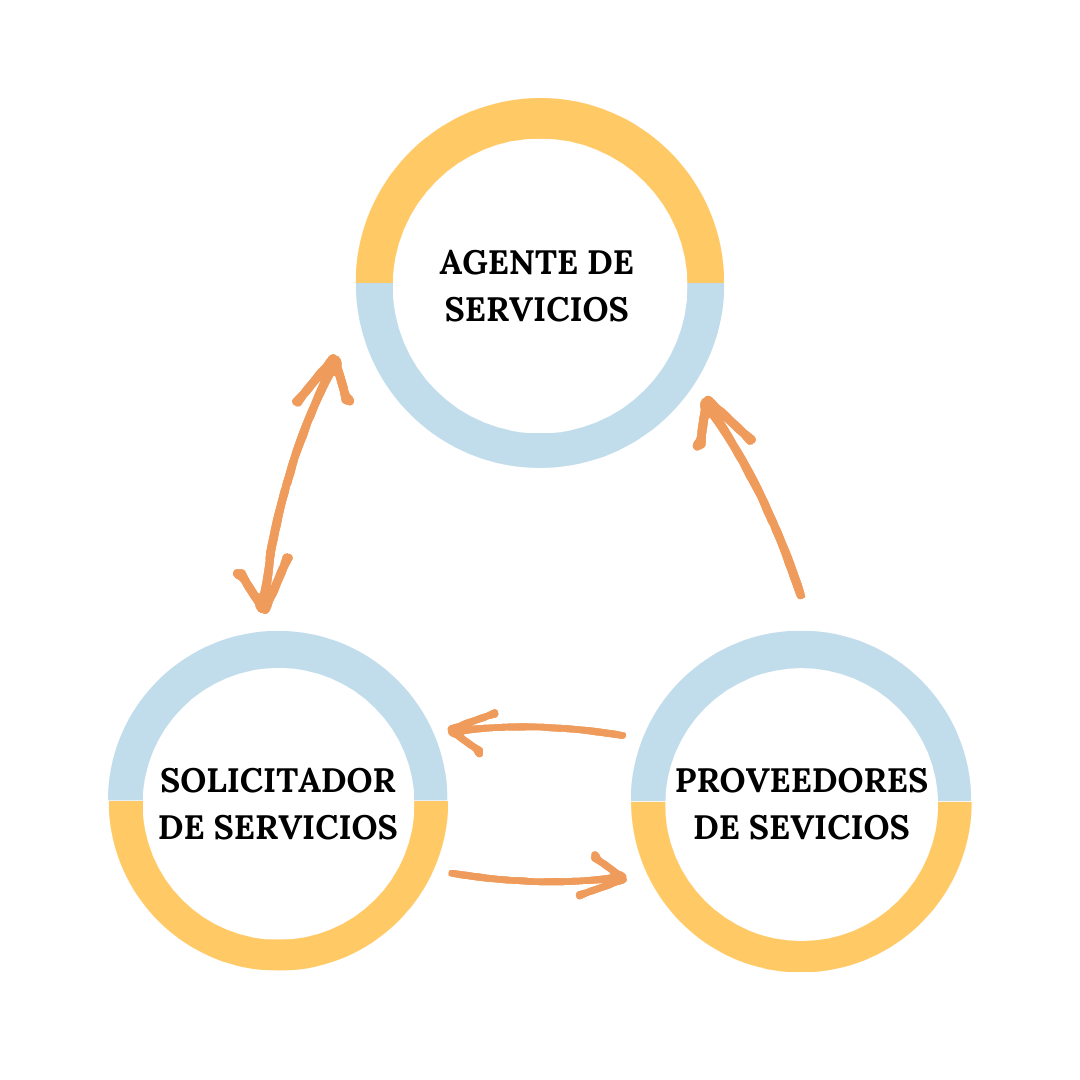
\includegraphics[width=0.8\linewidth]{2/brokerage.png} 
			\caption{Patr\'on arquitect\'onico en servicios web. }
			\label{fig:brokerage}
		 \end{center} 
	 \end{figure} 
		
%%		\item[Otros Patrones] 	En \LI \cite{Limoncelli2014}, el autor presenta una clasificaci\'on basada en patrones. Estos patrones forman parte de la estructura de los sistemas distribuidos, considere que los mismos est\'an compuesto por m\'ultiples componentes que aportan la funcionalidad que presentan los sistemas distribuidos, como la disponibilidad  y escalamiento de servicios. Se detallan tres patrones en particular: 
		
	%%		\item  Balanceador de carga con múltiples réplicas (\textit{backend})
			
%%			Los patrones que se muestran a partir de este, son parte de la estructura de los sistemas distribuidos presentados en \cite{Limoncelli2014}. En el patrón de composición del balanceador de carga con múltiples réplicas , ver la Figura \ref{fig:LoadBalance}, las solicitudes se envían al servidor del equilibrador de carga. Para cada solicitud, selecciona un \textit{{\gls{backends}}} y se reenvía la solicitud allí. La respuesta vuelve al servidor del equilibrador de carga, que a su vez la transmite al solicitante original.  Una solicitud enviada a cualquier réplica debería producir la misma respuesta.
			
%			\index{patrones!Balanceador de carga con múltiples réplicas de \textit{backend}}
			
			
			
	%		\begin{figure}  \begin{center}[h]%
		%		\includegraphics{loadBalancer.png} 				\caption{Balanceador de Cargas. Tomado de \LI}  				\label{fig:LoadBalance}  		 \end{center} \end{figure} 
			
			
			
%			\item  Servidor con varios réplicas
%			\index{patrones!Servidor con varios backends}
%			El siguiente patrón de composición es un servidor con múltiples réplicas o \textit{backends}. El servidor recibe una solicitud, envía consultas a muchos servidores backend y redacta la respuesta final combinando esas respuestas. Este enfoque se utiliza normalmente cuando la consulta original se puede descomponer  en una serie de consultas independientes que se pueden combinar para formar la respuesta final.
			
			
%			La Figura \ref{fig:ServerBackend}a ilustra cómo un motor de búsqueda simple procesa una consulta con la ayuda de múltiples backends. La interfaz recibe la solicitud. Transmite la consulta a muchos servidores backend.
			
			% 	\marginnote[-2.2cm]{
				%	\begin{kaobox}[frametitle= B\'usqueda en servidores replicados ]
					%		Si la b\'usqueda es textual, el corrector ortográfico responde con información para que el motor de búsqueda sugiera ortografías alternativas. Los backends de búsqueda de imágenes y web responden con una lista de sitios web e imágenes relacionadas con la consulta.  Una vez que se reciben las respuestas, la interfaz utiliza esta información para construir el HTML que forma la página de resultados de búsqueda para el usuario, que  se envía como respuesta.
					
					% 	\end{kaobox}   } 
			
%			\begin{figure}  \begin{center}[h]  				\includegraphics[width=0.8\textwidth]{ServerBackend.png} 				\caption{Servidores Replicados. Tomado de \LI}  				\label{fig:ServerBackend}  			 \end{center} \end{figure} 
			
			
			
%			La Figura \ref{fig:ServerBackend}b ilustra la misma arquitectura con backends replicados y con equilibrio de carga. Se aplica el mismo principio, pero el sistema puede escalar y sobrevivir mejor a las fallas.
			
%			\item Árbol de servidores
%			\index{patrones!Árbol de servidores}
%			El otro patrón de composición fundamental es el árbol de servidores. Como ilustra la Figura \ref{fig:ServerTree}, en este esquema varios servidores trabajan en cooperación con uno como la raíz del árbol, los servidores padres debajo de él y los servidores hoja en la parte inferior del árbol. 
			
%%			\marginnote[-4.2cm]{
%%				\begin{kaobox}[frametitle= Consultas en \'arbol de servidores ]
%%					Este patrón se utiliza para acceder a un gran conjunto de datos o corpus. Cada hoja almacena una fracción de los datos. 	 	La raíz recibe la consulta original y la reenvía a los padres, quienes la reenvían  a los servidores hoja. Cada hoja envía sus hallazgos a los padres, que clasifican y filtran los resultados antes de enviarlos a la raíz. La raíz toma las respuestas, combina los resultados y responde.
%%		 			\end{kaobox} 	 	} 
			
			
%		\begin{figure}  \begin{center}[h]								
%				\includegraphics[width=0.8\textwidth]{ServerTree.png}			\caption{\'Arbol de Servidores. Tomado de \LI} 				\label{fig:ServerTree} 			 \end{center} \end{figure} 
			
			

\begin{tcolorbox}
	[colback=red!5!white,colframe=red!75!black,fonttitle=\bfseries,title=  Brokerage]
	Puede leer m\'as de este tema en:
	\href{https://www.redhat.com/en/topics/cloud-native-apps/service-brokers}{Red Hat }  %%y en  \href{https://www.ibm.com/docs/en/was/9.0.5?topic=architecture-web-services-approach-service-oriented#:~:text=The%20service%20broker%2C%20also%20known,the%20scope%20of%20the%20broker}{Brokerage en IBM}.
\end{tcolorbox}
\end{description}



%%\section{\texttt{Soluciones basadas en middleware}}
%%La tarea del \gls{middleware} es proporcionar un nivel superior abstracción de programación para el desarrollo de sistemas distribuidos y, con las capas,  abstraer la heterogeneidad en la infraestructura subyacente para promover  interoperabilidad y portabilidad. Adem\'as de la soluciones de middleware presentados ,  también  hay arquitecturas más complejas como las siguientes: 
%%	\begin{itemize}
	%	\item Objetos Distribuidos: Corba, Java RMI
	%	\item Componentes distribuidos: Fractal
	%	\item Servidores de aplicaciones: Sun EJB, JBoss
	%	\item Servicios Web: Apache Axis
	%	\item Publicación-suscripción: Event Service, JMS
	%	\item Colas de mensajes: Websphere MQ
	%	\item Peer-to-peer: PASTRY, Tapestry, OceanStore, Gnutella
%%	\end{itemize}

%%%%%%%%%%%%%%%%%%%%%%%%%%%%%%%%%%%%%%%%
\section{Caso de Estudio: Sistema de Nombres de Dominio}
\index{DNS}
\index{caso de estudio!Sistema de Nombres de Dominio}
\label{cap:DNS}

El sistema de Nombres de Dominios (DNS, Domain Name Systems)  es un sistema de nombres que asigna nombres a otros datos, como direcciones IP, información de enrutamiento de correo y más. Es una base de datos distribuida  cuya finalidad es  permitir el control local de los segmentos de la base de datos general, los datos de cada segmento están disponibles en toda la red a través de un esquema cliente/servidor   \cite{Liu2011} \cite{Dostalek2006}.  La robustez y el rendimiento  adecuado del DNS se logran mediante la replicación de servidores  y el almacenamiento de datos en caché. 

DNS también es un sistema cliente-servidor, con clientes DNS consultando servidores DNS para recuperar datos almacenados en esa base de datos distribuida. Los clientes DNS  se denominan \gls{resolutores}, mientras que los servidores DNS a veces se denominan \gls{servidores de nombres}.
Toda la base de datos (o sistema de archivos) se representa como un árbol invertido, con el nodo raíz en la parte superior. Cada nodo del árbol tiene una etiqueta de texto que identifica el nodo en relación con su padre, ver Figura \ref{fig:DNS}.
En la Figura \ref{fig:DNS} se visualiza la estructura del árbol que caracteriza al DNS. Cada nodo representa nodos y las hojas pueden ser nodos o recursos. Los nodos de ubicados a la izquierda se refieren a los dominios genéricos: com, edu, org, gov; los nodos hacia la derecha se muestra los servidores de nombres dedicados a paises, por ejemplo: ac, al, co, pe, ve, entre otros. 

			
		\begin{figure} 
			 \begin{center}									
			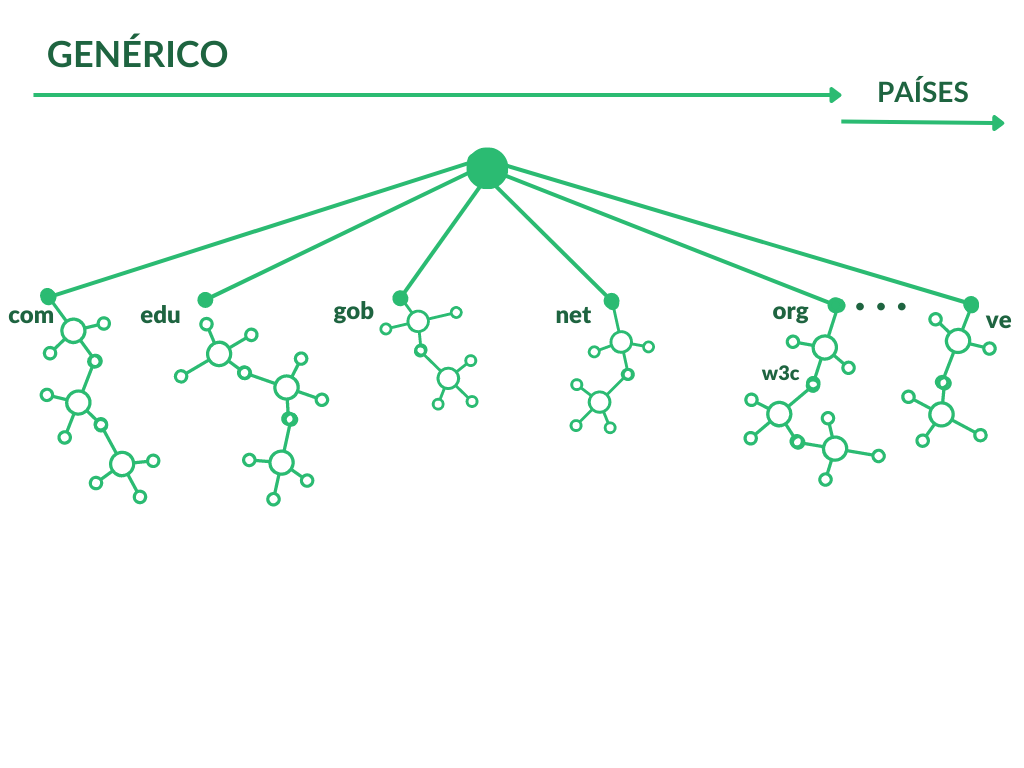
\includegraphics[width=0.8\linewidth]{2/DNS.png}		
			\caption{Sistemas de Nombres de Dominio. }
			\label{fig:DNS} 		
		 \end{center}
	  \end{figure} 

\subsection{Términos asociados al DNS}

\paragraph{Dominio.}  Refiriendosno a la  Figura \ref{fig:DNS}, cada nodo es  la raíz de un nuevo subárbol del árbol general. Cada uno de estos subárboles representa una partición de la base de datos general: un \textbf{dominio} en el DNS. Cada dominio o directorio se puede dividir en particiones adicionales, llamadas \textbf{subdominios}, como los subdirectorios de un sistema de archivos. Los subdominios, como los subdirectorios, se dibujan como elementos secundarios de sus dominios principales. Por ejemplo, en la Figura \ref{fig:DNS}, el dominio \textbf{org} y el subdominio \textbf{w3c}.
\index{dominio}


\paragraph{Espacio de nombres de dominio.}  La base de datos distribuida de DNS está indexada por nombres de dominio. El servicio intentará buscar un nombre válido, aunque se demuestre que ese nombre no corresponde a ningún objeto, es decir, que no poseé algún vinculo.  Cada nombre de dominio es esencialmente solo una ruta en el árbol, llamado \textbf{espacio de nombres de dominio}. 
\index{espacio de nombres de dominio}
Entonces, un dominio es  un subárbol del espacio de nombres del dominio. El nombre de dominio de un dominio es el mismo que el nombre de dominio del nodo en la parte superior del dominio, por ejemplo, la parte superior del subarbol \textit{\textbf{w3.org/}} es un nodo de nombre \textit{\textbf{w3.org/}}. Y un \textbf{espacio de nombres} es la colección de todos los nombres válidos reconocidos por un servicio en particular. El nombre de dominio completo de cualquier nodo en el árbol es la secuencia de etiquetas en la ruta desde ese nodo hasta la raíz. Ejemplo {\textbf{https://www.w3.org/}}, sería la ruta para la hoja principal, dentro del subárbol \textbf{org} de la Figura \ref{fig:DNS}.
\index{espacio de nombres}

\paragraph{Alias.}
Un \textbf{alias} es un nombre de dominio definido para denotar información sobre el servidor. Los alias permiten sustituir nombres más convenientes por otros menos complicados y permiten que distintas personas utilicen nombres alternativos para la misma entidad.
\index{alias}

\paragraph{Nombres de Dominios.}\textbf{Nombres de dominios} es un espacio de nombres para el cual existe una única autoridad administrativa general responsable de asignar nombres dentro de él. Esta autoridad tiene el control general de qué nombres pueden vincularse dentro del dominio, pero también puede delegar esta tarea. Los dominios en DNS son colecciones de nombres de dominio; sintácticamente, el nombre de un dominio es el sufijo común de los nombres de dominio que contiene, pero por lo demás no se puede distinguir, por ejemplo, de un nombre de computadora.
\index{nombres de dominio}
 
%%%%%%%%%%%%

\paragraph{Resolución} 
\index{resolución}
El proceso de obtención de una dirección de Internet a partir de un nombre de sistema principal se conoce como \textbf{resolución de nombres}.  La resolución de nombres es un proceso iterativo o recursivo mediante el cual un nombre se presenta repetidamente a contextos de nombres para buscar los atributos a los que se refiere. 

El proceso de localizar datos de nombres en más de un servidor de nombres para resolver un nombre se llama \textbf{navegación}. El software de resolución de nombres de clientes realiza la navegación en nombre del cliente. Se comunica con los servidores de nombres según sea necesario para resolver un nombre.  
Los modelos de navegación que soporta el DNS son los siguientes \cite{Coulouris2011}:

\begin{itemize}
	\item Navegación Iterativa desde el cliente.
	Para resolver un nombre, un cliente presenta el nombre al servidor de nombres local, que intenta resolverlo. Si el servidor de nombres local tiene el nombre, devuelve el resultado inmediatamente. Si no es así, sugerirá otro servidor que podrá ayudar. La resolución procede en el nuevo servidor, con más navegación según sea necesario hasta que se localiza el nombre o se descubre que no está vinculado, ver esquema en la Figura \ref{fig:DNS-inter}
	
	
	\begin{figure}  
		\begin{center}									
		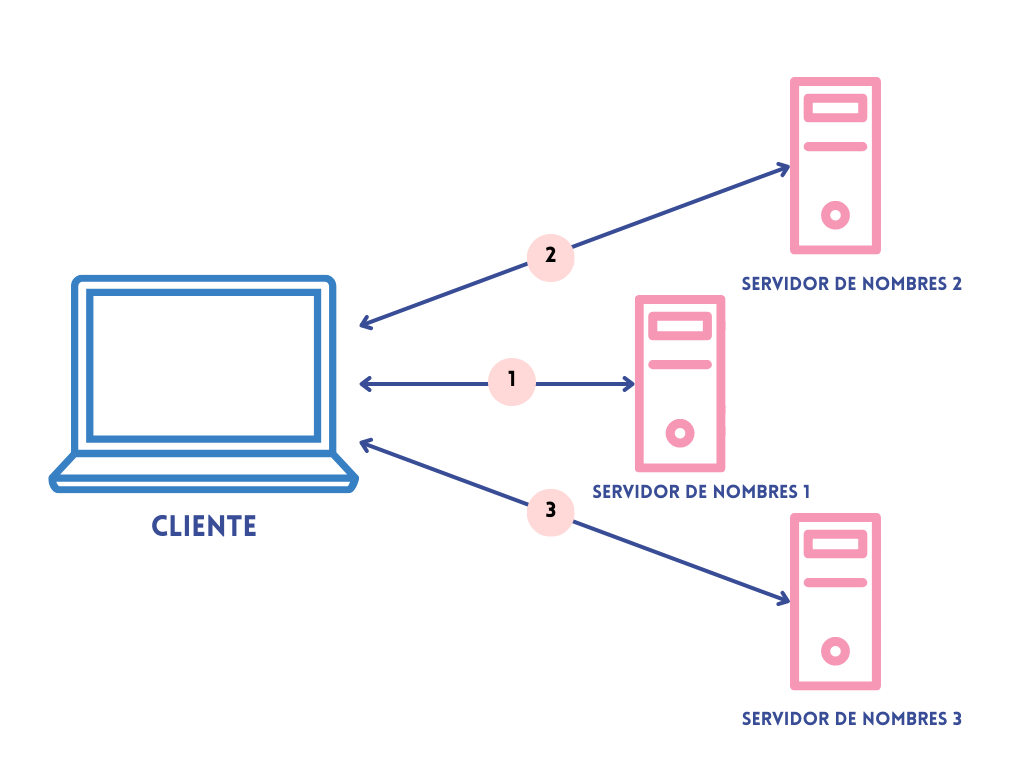
\includegraphics[width=0.8\linewidth]{2/DNS-inter.png}		
		\caption{DNS: Búsqueda Interactiva desde el cliente. }
		\label{fig:DNS-inter} 		
	 \end{center} 
 \end{figure} 
	
	\item Navegación Iterativa controlada por el servidor.
	
	En la Figura \ref{fig:DNS-inter-serv}, se muestra otra alternativa al modelo de navegación iterativa, en la que un servidor de nombres coordina la resolución del nombre y devuelve el resultado al  usuario.  Bajo la navegación iterativa controlada por el servidor,  el cliente puede elegir cualquier servidor de nombres. Este servidor se comunica iterativamente o por multidifusión con sus pares, como si fuera un cliente.
	\begin{figure}  
		\begin{center}									
		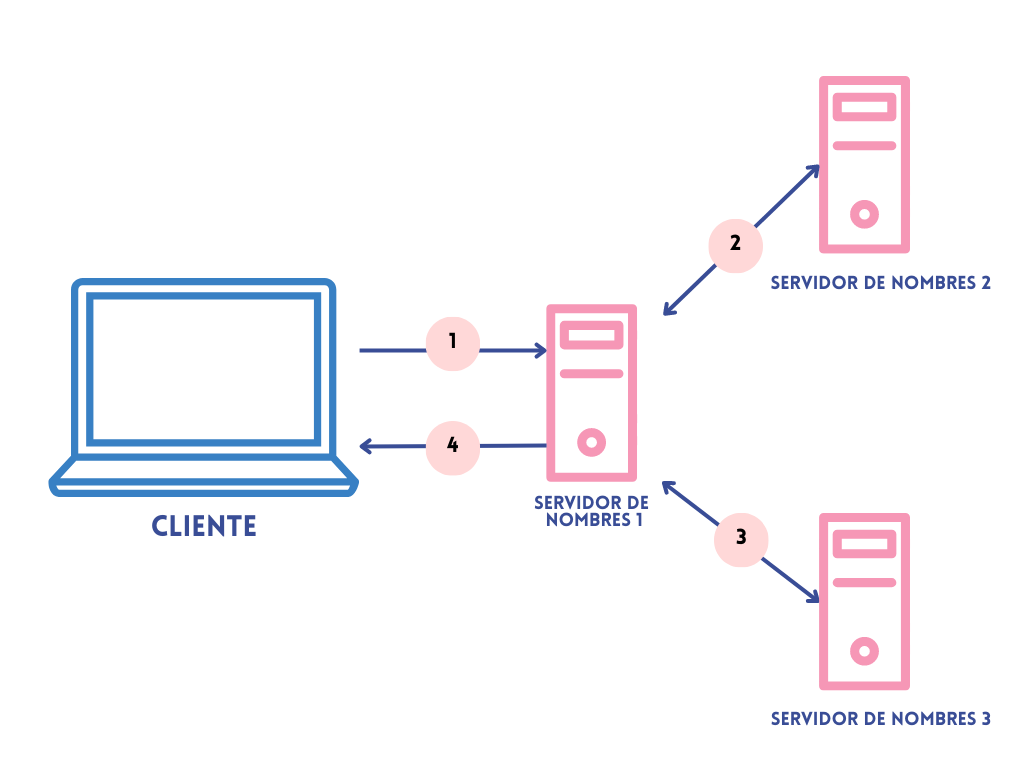
\includegraphics[width=0.8\linewidth]{2/DNS-inter-serv.png}		
		\caption{DNS: Búsqueda Interactiva desde el servidor. }
		\label{fig:DNS-inter-serv} 		
	 \end{center} 
 \end{figure} 
		
	\item Navegación Recursiva controlada por el servidor.
	  En la navegación recursiva controlada por el servidor, ver Figura \ref{fig:DNS-recur}, el cliente  contacta a un solo servidor. Si este servidor no almacena el nombre, el servidor contacta a un compañero que almacena un prefijo  del nombre, que a su vez intenta resolverlo. Este procedimiento continúa recursivamente hasta que se resuelve el nombre.
	
		\begin{figure}  
			\begin{center}									
		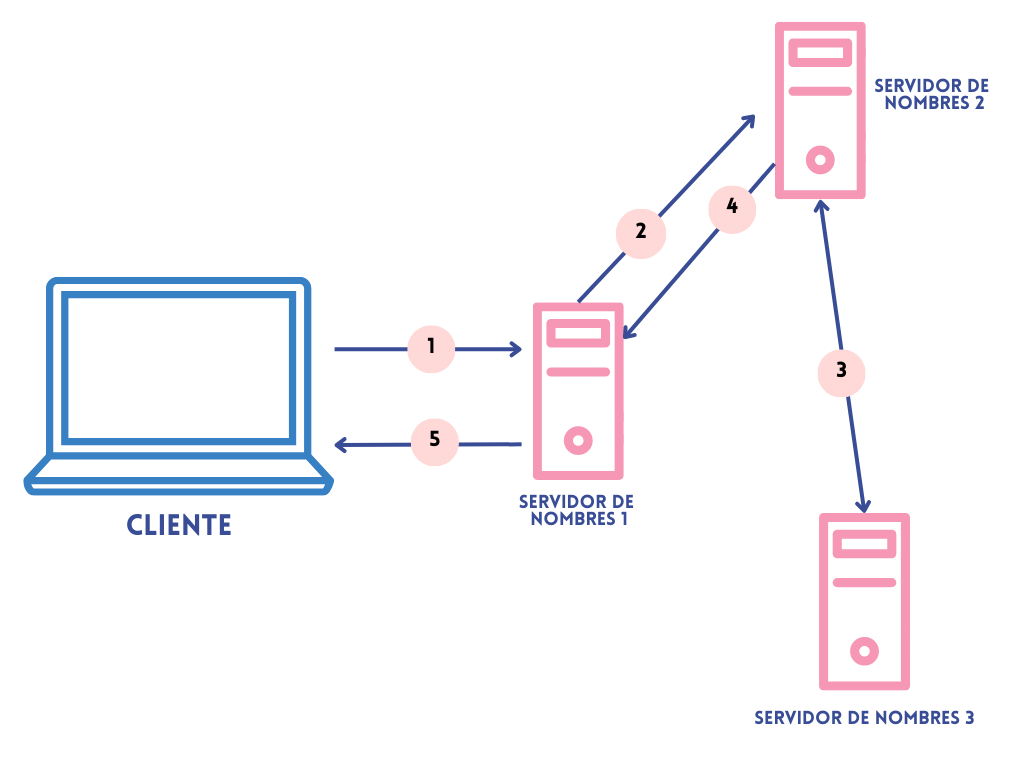
\includegraphics[width=0.8\linewidth]{2/DNS-recur.png}		
		\caption{DNS: Búsqueda Recursiva desde el servidor. }
		\label{fig:DNS-recur} 		
	 \end{center} 
 \end{figure} 
\end{itemize}


%%%%%%%

\paragraph{Ejemplo de una resolución de nombres}

En el DNS,  el software de resolución de nombres de clientes y  servidores mantienen un \textbf{caché} de los resultados de resoluciones de nombres anteriores. Cuando un cliente solicita una búsqueda de nombre, el software de resolución de nombres consulta su caché. Si contiene un resultado reciente de una búsqueda anterior del nombre, lo devuelve al cliente; de lo contrario, se pone a buscarlo desde un servidor. El almacenamiento en caché es clave para el rendimiento de un servicio de nombres y ayuda a mantener la disponibilidad tanto del servicio de nombres como de otros servicios a pesar de las caídas del servidor de nombres.
\begin{figure}  
	\begin{center}									
	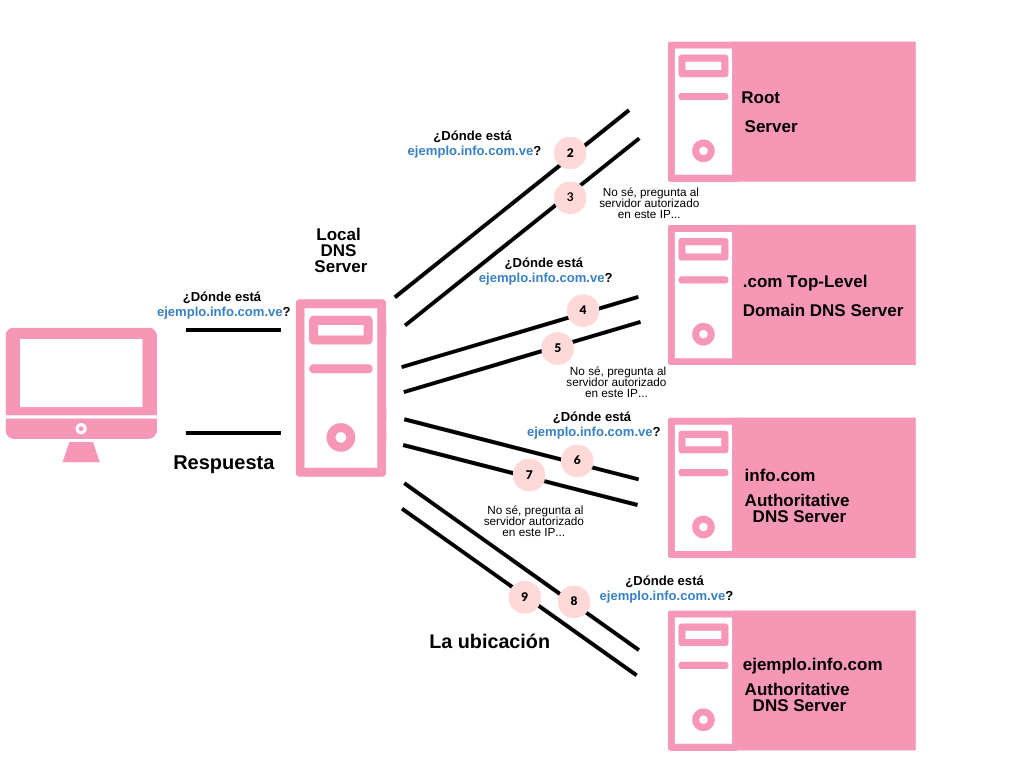
\includegraphics [width=0.8\linewidth]{2/DNS-busq.png}		
	\caption{DNS: Ejemplo de una búsqueda. }
	\label{fig:DNS-busq} 		
 \end{center} 
\end{figure} 


En la Figura \ref{fig:DNS-busq} se muestra  muestra el proceso de resolución de la dirección de un host  en un dominio. El servidor de nombres local consulta a un servidor de nombres raíz la dirección de \textit{ejemplo.info.com.ve} y se remite a los servidores de nombres \textbf{ve}. El servidor de nombres local le pregunta a un servidor de nombres \textbf{ve} la misma pregunta, y se remite a los servidores de nombres \textbf{com.ve}. El servidor de nombres \textbf{com.ve} remite el servidor de nombres local a los servidores de nombres \textbf{info.com.ve}. Finalmente, el servidor de nombres local
pide la dirección a un servidor de nombres \textbf{info.com.ve} y obtiene la respuesta.

	




%%%%%%%%%

%?` Que pasa cuando se envía una solicitud a un servidor?  
%Cuando los navegadores envían solicitudes a los servidores de archivos HTML, esos archivos HTML a menudo contienen elementos <link> que hacen referencia a hojas de estilo CSS externas y elementos <script> que hacen referencia a scripts JavaScript externos. Es importante saber el orden en que el navegador analiza esos archivos a medida que el navegador carga la página:

%El navegador analiza primero el archivo HTML, y eso hace que el navegador reconozca cualquier referencia de elemento <link> a hojas de estilo CSS externas y cualquier referencia de elemento <script> a scripts. A medida que el navegador analiza el HTML, envía solicitudes de regreso al servidor para cualquier archivo CSS que haya encontrado de los elementos <link>, y cualquier archivo JavaScript que haya encontrado de los elementos <script>, y de esos, luego analiza el CSS y JavaScript . El navegador genera un árbol DOM en memoria a partir del HTML analizado, genera una estructura CSSOM en memoria a partir del CSS analizado y compila y ejecuta el JavaScript analizado. A medida que el navegador construye el árbol DOM y aplica los estilos del árbol CSSOM y ejecuta JavaScript, se dibuja una representación visual de la página en la pantalla y el usuario ve el contenido de la página y puede comenzar a interactuar con él.

%En una aplicación web Ajax, no se interrumpe el usuario en interacciones con la aplicación web. El motor de Ajax o el intérprete JavaScript permite que el usuario interactúe con la aplicación web independientemente del transporte HTTP procedente del servidor o que tenga el servidor como destino representando la interfaz y gestionando las comunicaciones con el servidor en nombre del usuario. 

%%%%%%%%%%%%%%%%%%%%%%%%%%%%%%%%%%%


